\documentclass[handout]{beamer}
%\documentclass[notes]{beamer}
\usepackage{pgfpages}
%\setbeameroption{show notes on second screen}
%\setbeamertemplate{note page}[plain]
\usepackage{minted}

\usetheme{UiB}
\setbeamertemplate{navigation symbols}{}
\usepackage{quantikz}
\usepackage{booktabs}
\usepackage{inconsolata}
\usepackage{physics}
\usetikzlibrary{shapes}

\newcommand{\code}[1]{\texttt{#1}}

\newcommand{\source}[1]{%
    \setbeamertemplate{footnote}[unnumbered]%
    \footnotetext{#1}%
}

\title{Quantum Computing (Lab)}
\author{Incudini Massimiliano \\ Alessandra Di Pierro}
\institute{Università degli Studi di Verona}
\date{\today}

\begin{document}

\section{Lecture 1}
\SectionPage{}

\begin{frame}{The scenario}
    
\includegraphics[width=\textwidth]{img/lec1/qc_landscape.png}
\end{frame}


\begin{frame}{The scenario}
    
\includegraphics[width=\textwidth]{img/lec1/qc_landscape_zoom.png}
\end{frame}

\begin{frame}{How to install}
\begin{itemize}
    \item<1-> \url{https://youtu.be/aYCjWymN_Hk}
    \item<2-> Windows, Mac, Linux
    \item<3-> Python 3 + Anaconda + pip + Qiskit
\end{itemize}
\end{frame}


\begin{frame}[fragile]{Check your installation}
\begin{minted}{Python}
import qiskit
qiskit.__qiskit_version__
# {'qiskit-terra': '0.16.1',
#  'qiskit-aer': '0.7.2',
#  'qiskit-ignis': '0.5.1',
#  'qiskit-ibmq-provider': '0.11.1',
#  'qiskit-aqua': '0.8.1',
#  'qiskit': '0.23.2'}
\end{minted}
\end{frame}


\begin{frame}{Qiskit platform}
\begin{itemize}
    \item<1-> \emph{Terra}: circuit definition
    \item<2-> \emph{Aer}: simulation and execution
    \item<3-> \emph{Ignis}: error mitigation and correction
    \item<4-> \emph{Aqua}: algorithms for machine learning, optimization, finance, chemistry
\end{itemize}
\end{frame}



\begin{frame}{The Quantum Circuit}
\begin{itemize}
    \item<1-> define the circuit (\code{QuantumCircuit})
    \begin{itemize}
        \item<2-> 1+ \code{QuantumRegister} (w/ optional name)
        \item<3-> 0+ \code{ClassicalRegister} (w/ optional name)
    \end{itemize}
    \item<4-> draw the circuit (method \code{draw} of \code{QuantumCircuit})
    \item<5-> add the gates (methods of \code{QuantumCircuit})
    \begin{itemize}
        \item<6-> \code{.x(qubit)}
        \item<8-> \code{.h(qubit)}
        \item<9-> \code{.cx(control qubit, target qubit)}
        \item<10-> \code{.rx(theta, qubit)}
        \item<11-> \code{.crx(theta, control qubit, target qubit)}
        \item<12-> optionally use indexes instead of qubit
        \begin{itemize}
            \item<13-> depends on the order you insert the registers
            \item<14-> be consistent w/ the notation
        \end{itemize}
    \end{itemize}
    \item<15-> add the measurements (method of \code{QuantumCircuit})
    \begin{itemize}
        \item<15-> \code{.measure(qubit, cbit)}
    \end{itemize}
\end{itemize}
\end{frame}


\begin{frame}[fragile]{The code (1)}
\begin{minted}{python}
from qiskit import *

# first circuit
qr = QuantumRegister(2, 'qreg')
qc = QuantumCircuit(qr)
qc.draw()

qc.h(qr[0])
qc.cx(qr[0], qr[1])
qc.rx(0.1, qr[1])
qc.draw()
\end{minted}
\end{frame}


\begin{frame}[fragile]{The code (2)}
\begin{minted}{python}
# second circuit
qra = QuantumRegister(2, 'qa')
qrb = QuantumRegister(2, 'qb')
cr = ClassicalRegister(2, 'creg')
qc = QuantumCircuit(qra, qrb, cr)
qc.cx(qra[0], qra[1])
qc.cy(qrb[0], qrb[1])
qc.cx(0, 1)
qc.cy(2, 3)
qc.measure(0, 0)
qc.draw()
\end{minted}
\end{frame}

\begin{frame}{Simulators}
\begin{itemize}
    \item<1-> \emph{Statevector simulator}: output the complex vector of amplitudes
    \item<2-> \emph{Unitary simulator}: output the complex matrix representing the transformation performed by your circuit
    \item<3-> \emph{``QASM" simulator}: mime the behaviour of the real hardware, output the distribution of the possible outcomes
    \begin{itemize}
        \item<4-> error due to probabilistic nature of the processing
        \item<5-> \(\neq\) noise (which can be simulated too)
    \end{itemize}
\end{itemize}
\end{frame}

\begin{frame}[fragile]{The code (3)}
\begin{minted}{python}
from qiskit import Aer
Aer.backends()

statevector_sim = Aer.get_backend('statevector_simulator')
unitary_sim = Aer.get_backend('unitary_simulator')
qasm_sim = Aer.get_backend('qasm_simulator')

qc = QuantumCircuit(2, 2)
qc.h(0)
qc.cx(0, 1)

result = execute(qc, backend=statevector_sim, shots=1).result()
    .get_statevector()
# array([0.70710678+0.j, 0.        +0.j, 
#        0.        +0.j, 0.70710678+0.j])

result = execute(qc, backend=unitary_sim, shots=1).result().get_unitary()
# array([[ 0.70710678+0.00000000e+00j,  0.70710678-8.65956056e-17j,
#          0.        +0.00000000e+00j,  0.        +0.00000000e+00j],
#        [ 0.        +0.00000000e+00j,  0.        +0.00000000e+00j,
#          0.70710678+0.00000000e+00j, -0.70710678+8.65956056e-17j],
#        [ 0.        +0.00000000e+00j,  0.        +0.00000000e+00j,
#          0.70710678+0.00000000e+00j,  0.70710678-8.65956056e-17j],
#        [ 0.70710678+0.00000000e+00j, -0.70710678+8.65956056e-17j,
#          0.        +0.00000000e+00j,  0.        +0.00000000e+00j]])

result = execute(qc, backend=qasm_sim, shots=1000).result().get_counts()
# {'00': 1000}

qc.measure(0, 0)
qc.measure(1, 1)
result = execute(qc, backend=qasm_sim, shots=1000).result().get_counts()
# {'00 00': 506, '11 00': 494}
\end{minted}
\end{frame}


\begin{frame}[fragile]{The code (4)}
\begin{minted}{python}
result = execute(qc, backend=unitary_sim, shots=1).result()
    .get_unitary()
# array([
#  [ 0.70710678+0.00000000e+00j,  0.70710678-8.65956056e-17j,
#    0.        +0.00000000e+00j,  0.        +0.00000000e+00j],
#  [ 0.        +0.00000000e+00j,  0.        +0.00000000e+00j,
#    0.70710678+0.00000000e+00j, -0.70710678+8.65956056e-17j],
#  [ 0.        +0.00000000e+00j,  0.        +0.00000000e+00j,
#    0.70710678+0.00000000e+00j,  0.70710678-8.65956056e-17j],
#  [ 0.70710678+0.00000000e+00j, -0.70710678+8.65956056e-17j,
#    0.        +0.00000000e+00j,  0.        +0.00000000e+00j]
# ])
\end{minted}
\end{frame}


\begin{frame}[fragile]{The code (5)}
\begin{minted}{python}
result = execute(qc, backend=qasm_sim, shots=1000).result()
    .get_counts()
# {'00': 1000}

qc.measure(0, 0)
qc.measure(1, 1)
result = execute(qc, backend=qasm_sim, shots=1000).result()
    .get_counts()
# {'00': 503, '11': 497}
\end{minted}
\end{frame}

\begin{frame}{Bloch sphere}
\begin{itemize}
    \item<1-> Visualize single qubit transformations
    \item<2-> \code{kaleidoscope} library
    \item<3-> input \(=\) vector representing the quantum state
    \item<4-> interactive!
\end{itemize}

\begin{center}
    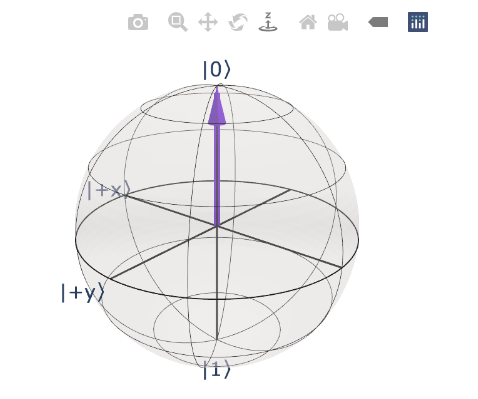
\includegraphics[width=0.5\textwidth]{img/lec1/bloch_sphere.png}
\end{center}
\end{frame}

\begin{frame}[fragile]{The code (6)}
\begin{minted}{python}
!pip install kaleidoscope
from kaleidoscope import bloch_sphere
from qiskit.quantum_info import Statevector
qc = QuantumCircuit(1)
figure = bloch_sphere(Statevector.from_instruction(qc))
figure.show()
\end{minted}
\end{frame}

% https://github.com/Qiskit/qiskit-tutorials/blob/master/tutorials/circuits_advanced/01_advanced_circuits.ipynb

\begin{frame}{Arbitrary initialization}
Encode a complex vector of \(2^n\) in a \(n\)-qubit register.
\end{frame}

\begin{frame}[fragile]{The code (7)}
\begin{minted}{python}
import numpy as np
amplitudes = np.array([1+0j, 2+2j, 3+4j, 6+0.55j])
amplitudes = amplitudes / np.linalg.norm(amplitudes)
# np.linalg.norm(amplitudes) = 0.9999999999999999
amplitudes = amplitudes / np.linalg.norm(amplitudes)
# np.linalg.norm(amplitudes) = 1.0

qc = QuantumCircuit(2)
qc.initialize(amplitudes)
\end{minted}
\end{frame}

\begin{frame}{Transpiling}
Given 
\begin{itemize}
    \item a circuit
    \item an universal set on ``known" gates
    \item a topology (pairs of adjacent qubits)
\end{itemize}
construct a circuit equivalent which can be run on the given configuration.

\only<2->{\bigskip Different (real) machines have different configurations, and the transpiling operation will lead to different circuits. }
\end{frame}

\begin{frame}[fragile]{The code (8)}
\begin{minted}{python}
qc = QuantumCircuit(2)

amp = array([0.11926544+0.j, 0.23853088+0.23853088j, 
             0.35779632+0.47706176j, 0.71559264+0.06559599j])
qc.initialize(amp)
qc.size() # 1

qc2 = transpile(qc, basis_gates=['u3', 'cx'])
qc2.size() # 6
\end{minted}
\end{frame}

\begin{frame}[fragile]{Execution on IBM machines}

Register on IBMQ, then visit \url{https://quantum-computing.ibm.com/account} and copy your token. Then execute (once): \medskip

\begin{minted}{python}
from qiskit import IBMQ
IBMQ.save_account('insert_token_here')
\end{minted}

\medskip Finally access your real backends through:\medskip

\begin{minted}{python}
IBMQ.load_account()
provider = IBMQ.get_provider()
# provider.backends() lists the available machines
backend = provider.get_backend('ibmq_santiago')
counts = execute(qc, backend, shots=1000).result().get_counts()
\end{minted}

\medskip Additional information on \url{github.com/Qiskit/qiskit-ibmq-provider}. 
\end{frame}

\begin{frame}{OpenQASM format}
Intermediate representation for quantum instructions. 

\only<2->{\bigskip Most circuit-based quantum computing framework can import and export from/to OpenQASM.}

\only<3->{\bigskip Try method \code{.qasm} of \code{QuantumCircuit}}
\end{frame}

\begin{frame}{Your turn!}
\begin{itemize}
    \item<1-> Check your Qiskit installation!
    \item<2-> Define the circuits implementing the Bell states, simulate and execute them with any backend seen so far (including real machines)
    \item<3-> Tell me: how much the circuit size for arbitrary initialization grows when the number of qubit grows?
    \item<4-> Try Deutsch-Jozsa (\url{qiskit.org/textbook/ch-algorithms/deutsch-jozsa.html})
    \item<5-> Open \url{qiskit.org/documentation/tutorials.html}
\end{itemize}
\end{frame}


\section{Lecture 2: \\ Quantum Protocols}
\SectionPage{}

\begin{frame}{Quantum Teleportation}

\bigskip

The IBM quantum computers currently do not support instructions after measurements, meaning we cannot run the quantum teleportation in its current form on real hardware. 

\bigskip

\begin{definition}[Principle of deferred measurement]
Measurements can always be moved from an intermediate stage of a quantum circuit to the end of the circuit.

If the measurement results are used at any stage of the circuit then the \alert{classically controlled operations} can be replaced by \alert{conditional quantum operations}.
\end{definition}

\end{frame}

\begin{frame}{Deferred Measurement}
 
 A consequence of the principle of deferred measurement is that \alert{measurement commutes with control}.
 
 \bigskip
 
\begin{center}
    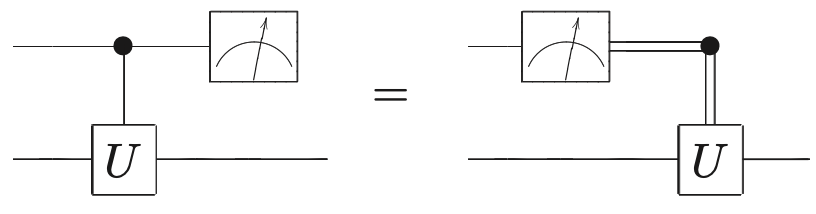
\includegraphics[width=0.85\textwidth]{img/DeferredMeasure.png}
\end{center}

\bigskip

\textbf{Exercise}

Prove the equality of the two circuits depicted above.


\end{frame}

\begin{frame}{Equivalent Teleportation Circuits}
 
\begin{center}
    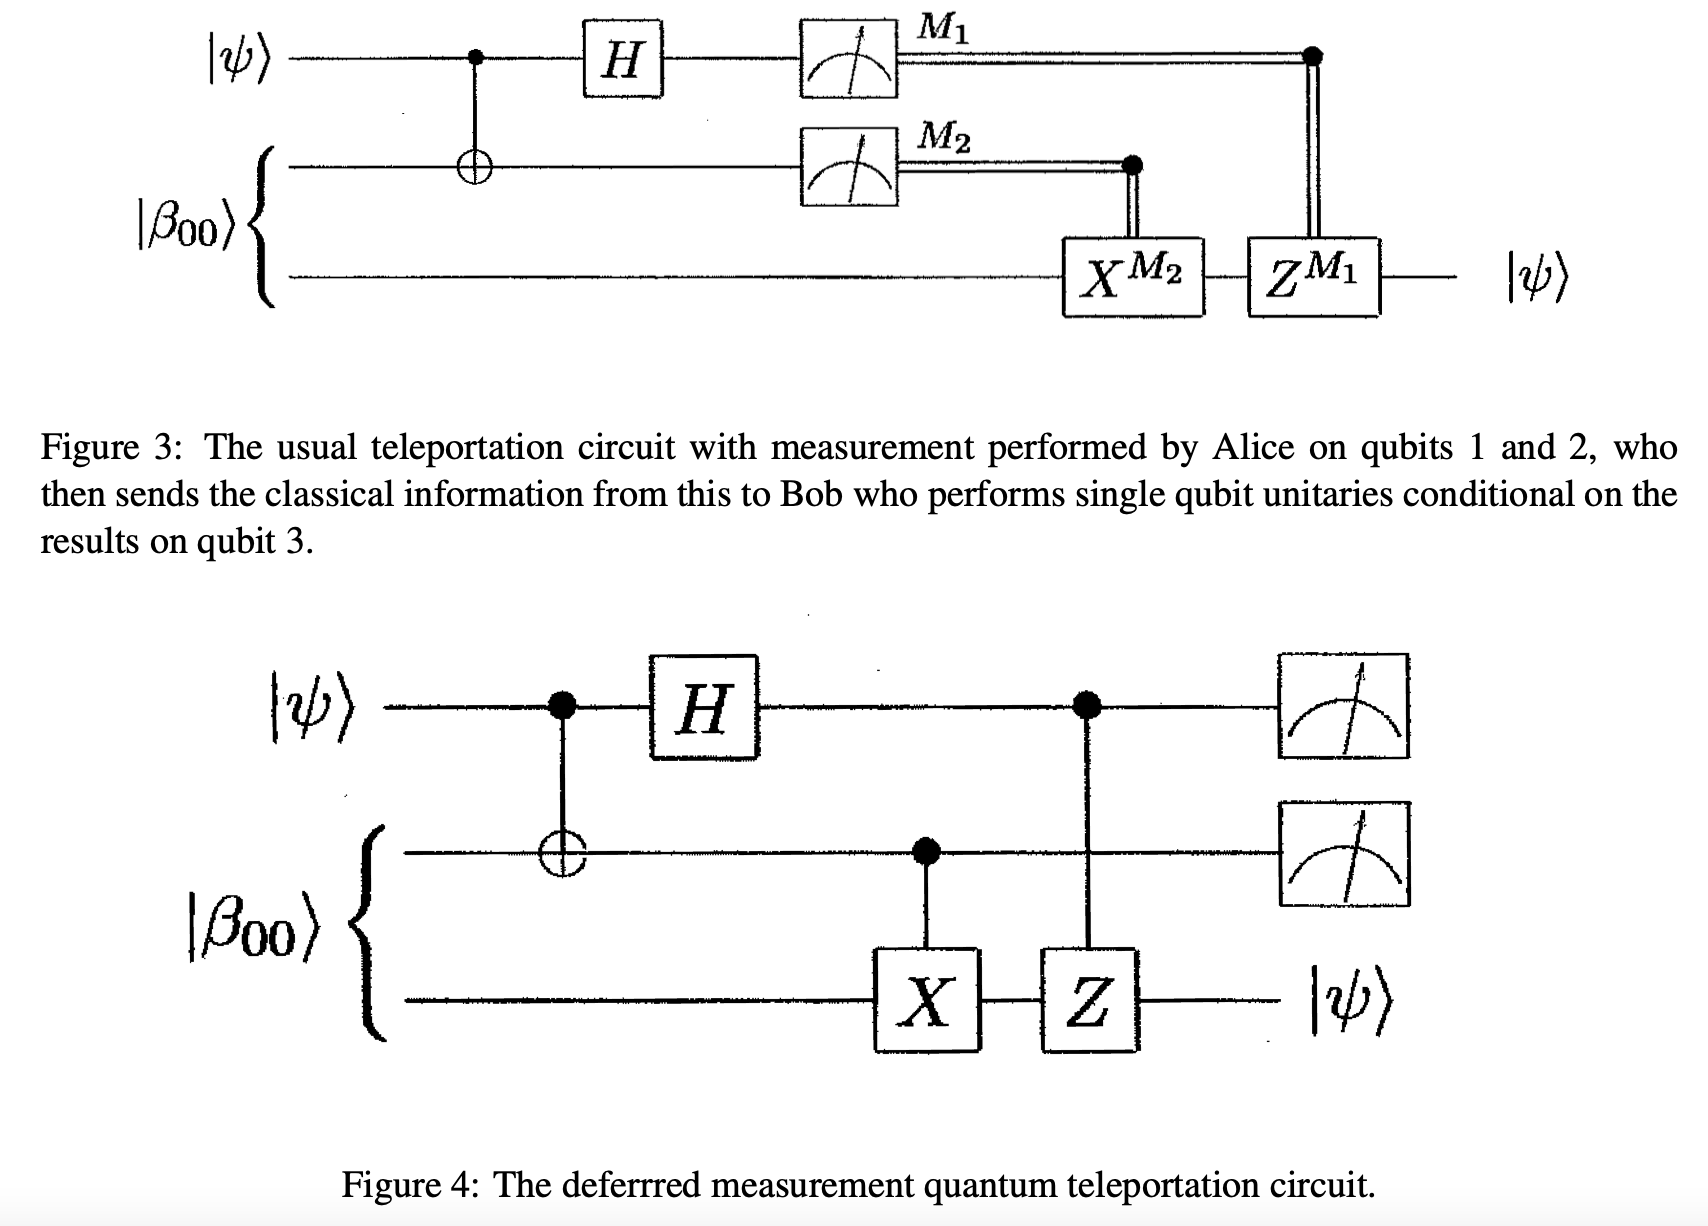
\includegraphics[width=0.80\textwidth]{img/EqivTelCircuits.png}
\end{center}
\end{frame}

\begin{frame}{Teleportation as State Transfer}
We are only interested in taking the input qubit $\psi$ to another location. We do not care what state we get in place of the original qubit at the sender. 

\begin{center}
    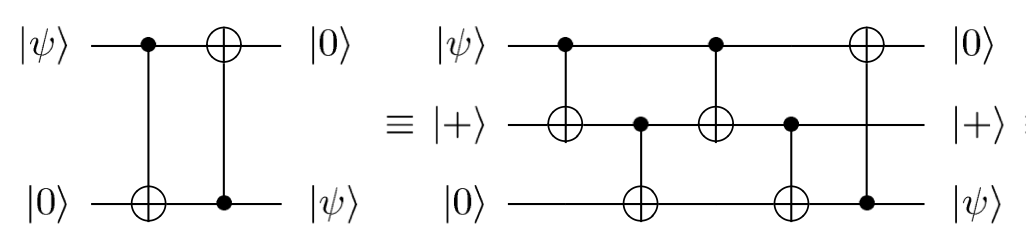
\includegraphics[width=0.80\textwidth]{img/state-transfer.png}
\end{center}

Other equivalent circuits:
\begin{center}
    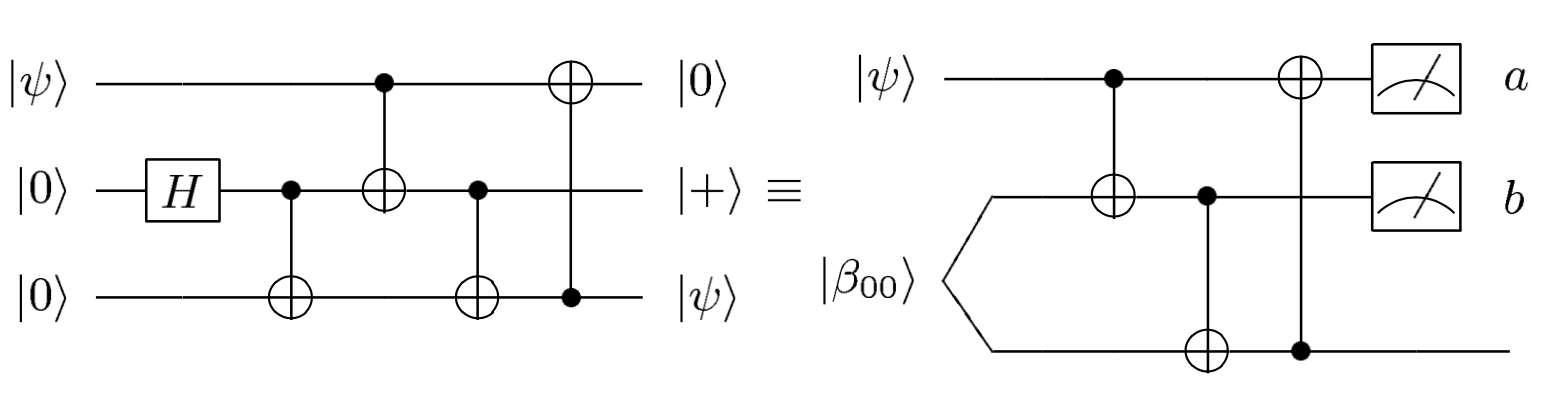
\includegraphics[width=0.80\textwidth]{img/Other-teleportation.png}
\end{center}
\end{frame}

\section{Exercise checking}
\SectionPage{}

% ============================================

\begin{frame}[fragile]{Exercise checking (1)}

\begin{itemize} 
\item Check your Qiskit installation
\end{itemize}

\begin{minted}{python}
import qiskit
qiskit.__qiskit_version__
\end{minted}

\bigskip No errors must appear (except the one regarding \code{matplotlib}, depending on the console you're using). 

\end{frame}

% ============================================

\begin{frame}[fragile]{Exercise checking (2)}

\begin{itemize} 
\item Define the circuits implementing the Bell states, simulate and execute them with any backend seen so far (including real machines)
\end{itemize}

\begin{minted}{python}
qc = QuantumCircuit(2, 2)
qc.h(0)
qc.cx(0, 1)

statevector_sim = Aer.get_backend('statevector_simulator')
statevector_result = execute(qc, backend=statevector_sim, shots=1)
    .result().get_statevector()

unitary_sim = Aer.get_backend('unitary_simulator')
unitary_result = execute(qc, backend=unitary_sim, shots=1)
    .result().get_unitary()
\end{minted}

\end{frame}


\begin{frame}[fragile]{Exercise checking (2)}

\begin{itemize} 
\item Define the circuits implementing the Bell states, simulate and execute them with any backend seen so far (including real machines)
\end{itemize}

\begin{minted}{python}
qc.measure([0, 1], [0, 1])
qasm_sim = Aer.get_backend('qasm_simulator')
qasm_result = execute(qc, backend=qasm_simulator, shots=1000)
    .result().get_statevector()

IBMQ.load_account()
santiago = IBMQ.get_provider().get_backend('ibmq_santiago')
counts = execute(qc, backend=santiago, shots=1000).result().get_counts()
\end{minted}

\end{frame}

% ============================================

\begin{frame}[fragile]{Exercise checking (3)}

\begin{itemize} 
\item How does the circuit size for arbitrary initialization grow when the number of qubit increases?
\end{itemize}

\begin{minted}{python}
from qiskit import * 
from qiskit.quantum_info.states.random import random_statevector

qubits = [1, 2, 3, 4, 5, 6, 7, 8]
sizes = []

for qubit in qubits:
	qc = QuantumCircuit(qubit)
	statevector = random_statevector(2**qubit)
	qc.initialize(statevector.data)
	qc2 = transpile(qc, basis_gates=['u3','cx'])
	sizes.append(qc2.size())
	
# sizes = [1, 6, 19, 48, 109, 234, 487, 996]
\end{minted}

\end{frame}


% ============================================

\begin{frame}[fragile]{Exercise checking (4)}

\begin{itemize} 
\item Try Deutsch-Jozsa
\end{itemize}

\bigskip See \url{qiskit.org/textbook/ch-algorithms/deutsch-jozsa.html}.

\end{frame}


\section{Quantum Teleportation}
\SectionPage{}

\begin{frame}{A note on Qiskit: which qubit is leftmost?}

\begin{center}
\begin{quantikz}[]
\lstick{\(\ket{\psi}\)}\qw
    & \gate[wires=3]{teleport}
    & \qw\rstick{\(\ket{b_1}\)} \\
\lstick{\(\ket{0}\)}\qw
    & \qw
    & \qw\rstick{\(\ket{b_2}\)} \\
\lstick{\(\ket{0}\)}\qw
    & \qw
    & \qw\rstick{\(\ket{\psi}\)}
\end{quantikz}
\end{center}

\bigskip At the beginning of the circuit the state is \( \ket{0} \otimes \ket{0} \otimes \ket{\psi} \)

\bigskip At the end of the circuit the state is \( \ket{\psi} \otimes \ket{b_2} \otimes \ket{b_1} \)

\end{frame}

% =====================================================

\begin{frame}[fragile]{The code (1)}

\begin{minted}[fontsize=\footnotesize]{python}
from qiskit.quantum_info.states.random import random_statevector
from qiskit import * \ import numpy as np

psi = random_statevector(2).data  
# array([0.75160912+0.04778984j, 0.49917654-0.42851213j])
qc = QuantumCircuit(3, 3)
qc.initialize(psi, 0)
sv_sim = Aer.get_backend('statevector_simulator')
statevector = execute(qc, sv_sim).result().get_statevector()
# array([0.75160912+0.04778984j, 0.49917654-0.42851213j,
#        0.        +0.j        , 0.        +0.j        ,
#        0.        +0.j        , 0.        +0.j        ,
#        0.        +0.j        , 0.        +0.j        ])
ket_zero = np.array([1, 0])
np.kron(np.kron(ket_zero, ket_zero), psi)
# array([0.75160912+0.04778984j, 0.49917654-0.42851213j,
#        0.        +0.j        , 0.        +0.j        ,
#        0.        +0.j        , 0.        +0.j        ,
#        0.        +0.j        , 0.        +0.j        ])
\end{minted}

\end{frame}


\begin{frame}{The protocol (1)}
\begin{quantikz}[]
\lstick[wires=2]{Alice}\qw
    & \gate{init(\ket{\psi})}
    & \qw \\
    \qw
    & \qw
    & \qw \\
\lstick{Bob}\qw
    & \qw
    & \qw
\end{quantikz}

\bigskip Alice own the qubit in state \(\ket{\psi} = \alpha \ket{0} + \beta \ket{1}\)
\end{frame}

% =========================================

\begin{frame}{The protocol (2)}
    
\begin{quantikz}[]
\lstick[wires=2]{Alice}\qw
    & \gate{init(\ket{\psi})}
    & \qw \\
    \qw
    & \gate[wires=2]{bell}
    & \qw\\
\lstick{\(\ket{0}\)}\qw
    & \qw
    & \qw
\end{quantikz}

\bigskip Alice and Bob shares a Bell state \(\frac{1}{\sqrt{2}} (\ket{00} + \ket{11})\)
\end{frame}

% =========================================

\begin{frame}[fragile]{Composed gates}

Hierarchical organization of the circuit

\begin{minted}{python}
def create_bell_circuit():
	bell_circuit = QuantumCircuit(2, name='bell')
	bell_circuit.h(0)
	bell_circuit.cx(0, 1)
	return bell_circuit

psi = random_statevector(2).data
qr = QuantumRegister(3, 'q')
crx = ClassicalRegister(1, 'crx')
crz = ClassicalRegister(1, 'crz')
qc = QuantumCircuit(qr, crx, crz)
qc.initialize(psi, qr[0])
qc.append(create_bell_circuit(), [qr[0], qr[1]])
\end{minted}
\end{frame}

% =========================================

\begin{frame}{The protocol (3)}
    
\begin{quantikz}[]
\lstick[wires=2]{Alice}\qw
    & \gate{init(\ket{\psi})}
    & \ctrl{1} 
    & \gate{H} 
    & \qw \\
    \qw
    & \gate[wires=2]{bell}
    & \targ{}
    & \qw
    & \qw\\
\lstick{\(\ket{0}\)}\qw
    & \qw
    & \qw
    & \qw
    & \qw
\end{quantikz}

\bigskip Alice applies CNOT and H, the state becomes
\begin{align*}
    \frac{1}{2} \Big( & \ket{00}(\alpha \ket{0} + \beta \ket{1}) \\
                    + & \ket{01}(\alpha \ket{1} + \beta \ket{0}) \\
                    + & \ket{10}(\alpha \ket{0} - \beta \ket{1}) \\
                    + & \ket{10}(\alpha \ket{1} - \beta \ket{0})\Big) 
\end{align*}
\end{frame}

% =========================================

\begin{frame}{The protocol (4)}
    
\begin{quantikz}[]
\lstick[wires=2]{Alice}\qw
    & \gate{init(\ket{\psi})}
    & \ctrl{1} 
    & \gate{H} 
    & \meter{}
    & \cw
    & \cwbend{2}\\
    \qw
    & \gate[wires=2]{bell}
    & \targ{}
    & \qw
    & \meter{}
    & \cwbend{1} \\
\lstick{\(\ket{0}\)}\qw
    & \qw
    & \qw
    & \qw
    & \qw
    & \gate{X}
    & \gate{Z}
    & \qw
\end{quantikz}

\bigskip Alice measures and send the two classical bits, Bob adjusts its qubit according to the received bits:
\begin{align*}
    00 & \to I \\
    01 & \to X \\
    10 & \to Z \\
    11 & \to ZX
\end{align*}
\end{frame}

% =========================================

\begin{frame}[fragile]{The code (2)}
\begin{minted}{python}
psi = random_statevector(2).data

qr = QuantumRegister(3, 'q')
crx = ClassicalRegister(1, 'crx')
crz = ClassicalRegister(1, 'crz')
qc = QuantumCircuit(qr, crx, crz)
qc.initialize(psi, qr[0])
qc.append(create_bell_circuit(), [qr[1], qr[2]])

qc.cx(qr[0], qr[1])
qc.h(qr[0])
qc.measure(qr[0], crz)
qc.measure(qr[1], crx)
qc.x(qr[2]).c_if(crx, 1)
qc.z(qr[2]).c_if(crz, 1)
\end{minted}
\end{frame}

\begin{frame}[fragile]{The code (3)}
\begin{minted}{python}
sv_sim = Aer.get_backend('statevector_simulator')
sv = execute(qc, sv_sim).result().get_statevector()
\end{minted}

\bigskip Is \code{sv} the state \( \ket{\psi} \otimes \ket{b_2} \otimes \ket{b_1} \)?
\end{frame}

% =========================================

\begin{frame}[fragile]{The code (4)}

What is we use deferred measurements? \bigskip

\begin{minted}{python}
qr = QuantumRegister(3, 'q')
crx = ClassicalRegister(1, 'crx')
crz = ClassicalRegister(1, 'crz')
qc = QuantumCircuit(qr, crx, crz)
qc.initialize(psi, qr[0])
qc.append(create_bell_circuit(), [qr[1], qr[2]])

qc.cx(qr[0], qr[1])
qc.h(qr[0])
qc.cx(qr[0], qr[2])
qc.cz(qr[1], qr[2])
qc.measure(qr[0], crz)
qc.measure(qr[1], crx)
\end{minted}
\end{frame}

% =========================================

\begin{frame}{Running on real quantum computers}

\begin{itemize}
    \item Deferred measurement is mandatory;
    \item How can I check if the state is exactly the one Alice wanted to send?
\end{itemize}
\end{frame}

\begin{frame}{Running on real quantum computers}

\begin{itemize}
    \item Deferred measurement is mandatory;
    \item How can I check if the state is exactly the one Alice wanted to send?
\end{itemize}

\bigskip
\begin{center}
\begin{quantikz}[]
\lstick{\(\ket{0}\)}\qw
    & \gate{init}
    & \gate[wires=3]{teleport}
    & \qw \\
\lstick{\(\ket{0}\)}\qw
    & \qw
    & \qw
    & \qw \\
\lstick{\(\ket{0}\)}\qw
    & \qw
    & \qw
    & \gate{init^{-1}}
    & \qw\rstick{\(\ket{0}\)}
\end{quantikz}
\end{center}

\qquad Check if the last qubit is zero

\end{frame}

% =========================================

\begin{frame}[fragile]{Inverse of \code{initialize} gate}

\begin{minted}{python}
from qiskit.extensions import Initialize
psi = random_statevector(2).data

init_gate = Initialize(psi)
init_gate.label = 'init'

inverse_init_gate = init_gate.gates_to_uncompute()

qc = QuantumCircuit(1)
qc.append(init_gate, [0])
qc.append(inverse_init_gate, [0])
sv = execute(qc, sv_sim).result().get_statevector()
# sv is ALMOST ket zero
\end{minted}

\end{frame}

% =========================================

\begin{frame}[fragile]{Inverse of \code{initialize} gate}

Be careful: \code{initialize} contains a non-linear \code{Reset} gate \bigskip

\begin{minted}{python}
init_gate = Initialize(psi)
init_gate.inverse() # error

inverse_init_gate = init_gate.gates_to_uncompute() # no reset
init_wo_reset = inverse_init_gate.inverse()

init_wo_reset.inverse() # ok
\end{minted}

\end{frame}

\begin{frame}{More on Quantum Teleportation}
Check this video of \emph{minutephysics}: \url{youtube.com/watch?v=dAaHHGHuy1c}
\end{frame}

\begin{frame}{Your turn!}
\begin{itemize}
    \item Demonstrate the equivalence of these circuits:
    \begin{center}
        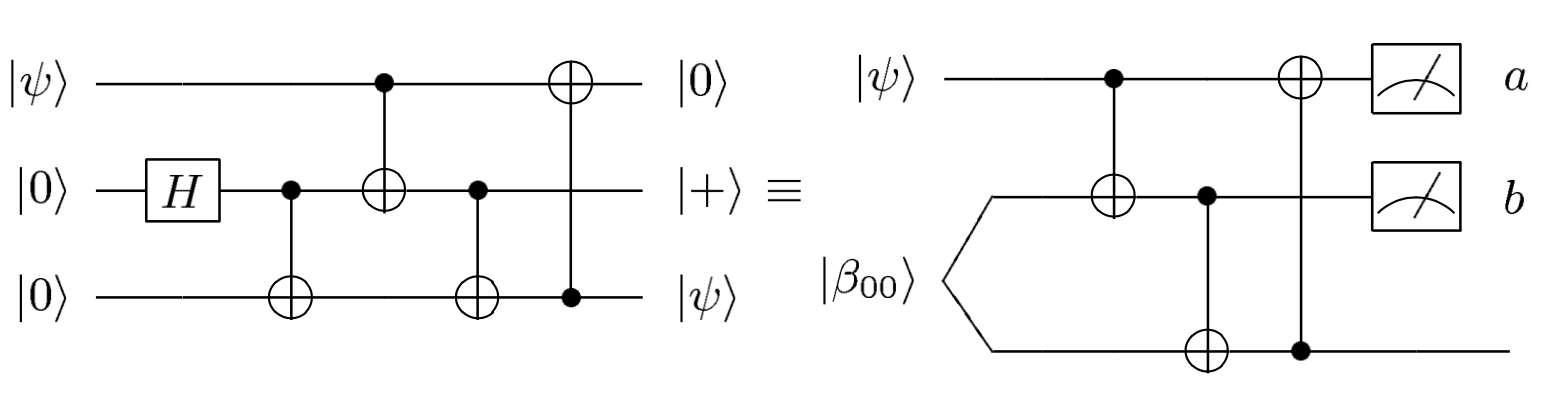
\includegraphics[width=0.80\textwidth]{img/Other-teleportation.png}
    \end{center}
    \item Run Quantum Teleportation
    \begin{itemize}
        \item \url{qiskit.org/textbook/ch-algorithms/teleportation.html}
        \item Explain how the network is used by Bob (Step 4) if the Bell state in input is $\frac{1}{\sqrt{2}}(\ket{01}+\ket{10})$.
    \end{itemize}
    \item Run Superdense Coding
    \begin{itemize}
        \item \url{qiskit.org/textbook/ch-algorithms/superdense-coding.html}
        \item Familiarize with the documentation!
    \end{itemize}
\end{itemize}

\end{frame}

% nota: eseguendo il circuito più volte il risultato dello statevector cambia, però facendo i conti sono i primi due qubit che cambiano e non il terzo
% controllare con metodo che fa 00psi, 01psi, 10psi, 11psi



\section{Lecture 3-4:\\ Applications to\\ Machine Learning}
\SectionPage{}

\begin{frame}{Aspect of QC that can improve ML}

Several algorithms for quantum computers have been proposed which improve the performance of machine learning software. Here we consider some \emph{classification} problem having \(N\) size of training set, \(M\) number of feature per sample. \bigskip

Samples $x \in \mathbb{R}^n$ are encoded through a piece of circuit called \emph{feature map} $U(x)$.

\end{frame}


\begin{frame}{Some approaches}
\begin{center}
\begin{tabular}{c c}
    Algorithm & Improvement \\ \midrule
    SWAP-test & Distance procedure from \(O(M)\) to \(O(\log(M))\)  \\[1em]
    QSVM & The quantum circuit act ``like" a kernel function  \\[1em]
    QNN & Sometimes lead to faster training  \\[1em]
\end{tabular}
\end{center}
\end{frame}

\begin{frame}{Swap-test}

Efficient procedure to calculate the inner product. Since the circuit depth linear in the number of qubits, it can lead to an exponential speed-up (depending on how you encode the data).

\begin{center}
\begin{quantikz}
\lstick{$\ket{0}$}      & \gate{H} & \ctrl{2} & \gate{H} & \meter{} \\
\lstick{$\ket{\psi_1}$} & \qw      & \swap{1} & \qw      & \qw \\
\lstick{$\ket{\psi_2}$} & \qw      & \swap{0} & \qw      & \qw \\
\end{quantikz}
\end{center}

\[p(\text{measure }0) = \braket{\psi_1}{\psi_2}\]

\only<2->{\bigskip \emph{Note}: \(\text{distance}(\psi_1, \psi_2)^2 = 2(1-\braket{\psi_1}{\psi_2}) \)}
\end{frame}


\begin{frame}{K-nearest neighbor classificator with swap-test}
\begin{enumerate}
    \item<1-> Consider some unlabelled instance \(\tilde{x}\) and some training set \((x_1, y_1); ...; (x_n, y_n)\) where \(y_i \in \{\ell_1, ..., \ell_m\}\)
    \item<2-> Calculate the inner product between \(\tilde{x}\) and any \(x_i\) through the swap-test;
    \item<3-> Pick the \(k\) elements whose inner product is bigger and their corresponding labels, infer \(\tilde{y}\) to be the most occurring label.
\end{enumerate}
\end{frame}


\begin{frame}[fragile]{Your turn!}
Build the swap-test circuit.

Build a classificator for IRIS problem, then calculate its accuracy. \bigskip

\begin{minted}{python}
from qiskit.ml.datasets import iris
sample_train, training_input, test_input, class_labels = 
    iris(training_size=40, test_size=10, n=4)
# len(training_input[key]) == 40 for key in ['A', 'B', 'C']
# len(test_input[key]) == 10 for key in ['A', 'B', 'C']

# fix qiskit.ml.datasets.iris code line 30: 
# test_size=test_size*len(class_labels)
\end{minted}
\end{frame}


\begin{frame}[fragile]{Your turn! (hint)}

\begin{minted}{python}
from heapq import nlargest
from operator import itemgetter
def most_common(lst): return max(set(lst), key=lst.count)

def quantum_classifier(x, training_set):
    k=3
    similarities = []
    for label in ['A', 'B', 'C']:
        for item in training_set[label]:
            the_ip = quantum_inner_product(x, item)
            similarities.append((the_ip, label))
    k_similarities = nlargest(k, similarities, key=itemgetter(0))
    _, k_labels = zip(*k_similarities)
    return most_common(k_labels)
\end{minted}
\end{frame}


\begin{frame}{More on swap-test classifier}

The Hadamard classifier (Schuld et al.) implements a whole classifier. 

\begin{center}
    \begin{quantikz}[]%
    \lstick{\(\ket{a}\)}\qw%
        & \gate{H}%
        & \ctrl{2}%
        & \gate{X}%
        & \ctrl{2}%
        & \qw%
        & \ctrl{2}%
        & \gate{H}%
        & \meter{discard 1} \\%
    \lstick{\(\ket{m}\)}\qw%
        & \gate{H}%
        & \qw%
        & \qw%
        & \ctrl{1}%
        & \gate{X}%
        & \ctrl{1} %
        & \ctrl{2}%
        & \qw\\%
    \lstick{\(\ket{d}\)}\qw%
        & \qw%
        & \gate{\tilde{x}}%
        & \qw%
        & \gate{x_1}%
        & \qw%
        & \gate{x_2}%
        & \qw%
        & \qw\\%
    \lstick{\(\ket{c}\)}\qw%
        & \qw%
        & \qw%
        & \qw%
        & \qw%
        & \qw%
        & \qw%
        & \targ{}%
        & \meter{}%
\end{quantikz}
\end{center}

\[p(\text{measure }\ket{c}\;0) = \begin{cases}
    <0.5, & d(\tilde{x}, x_1) < d(\tilde{x}, x_2) \\
    >0.5, & d(\tilde{x}, x_1) > d(\tilde{x}, x_2)
\end{cases} \]

\end{frame}


\begin{frame}{QSVM}
Sometimes data cannot be separated in the original feature space, but can be separated in another (higher dimensional) ones. 

\only<2->{\bigskip The embedding of data into a different space is called \emph{feature maps}. Once the data is embedded, the classification can be run into the higher dimensional space (NB: the only operation we care for is the inner product).}

\only<3->{\bigskip Each embedding of data into a quantum circuit act as a feature map, then the inner product is performed by the swap-test.}

\only<4->{\bigskip \emph{Difference with the previous classifier}: no performance improvement, potential accuracy improvement (depending on the efficacy of the feature map)}

\only<5->{\bigskip The procedure make sense only for feature map that cannot be simulated efficiently on classical hardware.}
\end{frame}


\begin{frame}[fragile]{Your turn!}
Try the QSVM. Check some feature map available on Qiskit documentation (find the meaning of \code{repetition} and \code{entanglement} parameters). Create a new feature map extending class \code{qiskit.aqua.components.feature\_maps.FeatureMap} (four qubit, one \code{RX} gate per each qubit - and feature of IRIS). \bigskip

\begin{minted}{python}
from qiskit.circuit.library import ZZFeatureMap
feature_map = ZZFeatureMap(feature_dimension=4, reps=1, entanglement='linear')
backend = Aer.get_backend('statevector_simulator')
quantum_instance = QuantumInstance(backend, shots=1))
qsvm = QSVM(feature_map, training_input, test_input)
result = qsvm.run(quantum_instance)
print(f'Testing success ratio: {result["testing_accuracy"]}')
\end{minted}
\end{frame}

\begin{frame}[fragile]{Parametrized circuits}
Circuit depending on some parameters.\bigskip

\begin{minted}{python}
theta = Parameter('theta')
qc = QuantumCircuit(1)
qc.rx(theta, 0)

# bind paramenters explicitly
qc2 = qc.bind_parameters({theta: 0.123})
qc2.draw()

# bind parameters when executing
execute(qc, backend=..., parameter_binds=[
    {theta: theta_val} for theta_val in [0.1, 0.2, 0.3])
\end{minted}
\end{frame}

\begin{frame}{Variational Quantum Classifier}
    
A variational quantum circuit contains parameterized gates whose values depend on some variables $\theta_1, ..., \theta_n$.

\begin{enumerate}
    \item Instantiate the circuit choosing random $\theta$s;
    \item Run the circuit and obtain output $y$;
    \item Use $y$ to compute a loss function and update $\theta$s accordingly.
\end{enumerate}

\bigskip\alert{Advantage}: The iterative optimization of the parameters allows us to circumvent the high-depth circuit.

\medskip\structure{Disadvantage}: No assurance of speedup. 
\end{frame}





\begin{frame}{Variational Quantum Classifier (2)}

\begin{center}
    \begin{quantikz}
    \lstick[wires=3]{$\ket{0}$} 
    & \gate[wires=3][2cm]{U(x)} & \gate[wires=3][2cm]{U(\theta)} & \meter{} \rstick[wires=3]{$y$} \\
    & \qw & \qw & \meter{}  \\
    & \qw & \qw & \meter{}  \\
    \end{quantikz}
\end{center}

\begin{itemize}
    \item input $x \in \mathbb{R}^n$ is encoded through \emph{feature map} $U(x)$;
    \item the state evolves through variational form $U(\theta)$;
    \item the parameters $\theta$s are chosen to minimize a certain loss function.
\end{itemize}

\end{frame}




\begin{frame}{Variational Quantum Classifier (3)}

Any variational circuit is a QNN. 
\begin{itemize}
    \item Mathematically, a QNN is a rather different object compared to classical NN;
    \item the analogy refers to:
    \begin{itemize}
        \item ``modular" nature of quantum gates in a circuit;
        \item use of tricks from training neural networks in the optimization of quantum algorithms.
    \end{itemize}
\end{itemize}

\begin{center}
    \scalebox{0.9}{
    \begin{quantikz}
        \qw
            & \gate{RY(\theta_1)} \gategroup[wires=3,steps=4,style={inner sep=-0.2pt}]{hidden layer 1}
            & \ctrl{1}           
            & \ctrl{2} 
            & \qw
            & \gate{RY(\theta_4)} \gategroup[wires=3,steps=4,style={inner sep=-0.2pt}]{hidden layer 2}
            & \ctrl{1}           
            & \ctrl{2} 
            & \qw 
            & \qw \\
        \qw 
            & \gate{RY(\theta_2)} 
            & \targ{}  
            & \qw      
            & \ctrl{1}
            & \gate{RY(\theta_5)} 
            & \targ{}  
            & \qw      
            & \ctrl{1}
            & \qw \\
        \qw 
            & \gate{RY(\theta_3)} 
            & \qw      
            & \targ{}  
            & \targ{}
            & \gate{RY(\theta_6)} 
            & \qw      
            & \targ{}  
            & \targ{}
            & \qw 
    \end{quantikz}}
\end{center}

\end{frame}


\begin{frame}{Barren plateau}

\begin{block}{Barren Plateau}
When minimizing the cost function, we might have exponentially vanishing gradients, known as barren plateau landscapes. In that case, the network cannot be efficiently trained.
\end{block}

\begin{itemize}
    \item Depends on the network architecture (Cerezo et al., 2020);
    \item Depends on the feature map (Abbas et al., 2020). 
\end{itemize}
\end{frame}


\begin{frame}[fragile]{Your turn!}
Try the VQC. \bigskip

\begin{minted}{python}
IRIS_FEATURES = 4
optimizer = ADAM(maxiter=100, lr=0.1)
feature_map = ZZFeatureMap(feature_dimension=IRIS_FEATURES)
var_form = TwoLocal(IRIS_FEATURES)
vqc = VQC(optimizer, feature_map, var_form, 
    training_input, test_input)

backend = Aer.get_backend('statevector_simulator')
quantum_instance = QuantumInstance(backend, shots=1)
result = vqc.run(quantum_instance)
\end{minted}
\end{frame}







\end{document}